\chapter{Método Proposto}
  
O método proposto se utiliza do GRASP, do ILS e da abordagem exata através da
programação linear inteira, pretendendo tirar proveito das vantagens de cada
uma dessas técnicas. A agilidade dos métodos heurísticos e a optimalidade do
método exáto.
  
Da mesma forma que as outras abordagens heurísticas esse novo algoritmo
consome pouco tempo computacional, em relação ao método exato e tem a capacidade
de escapar de mínimos locais.
  
O GRASP foi utilizado como a base do algoritmo onde a parte da construção
seguiu a sua definição padrão, com a geração de uma lista restrita de candidados
(LRC) e a posterior escolha aleatória entre esses elementos. A parte da busca
local foi adaptada para executar em conjunto com o ILS modificado. Para o ILS
foram definidos algumas estruturas de vizinhança que foram utilizadas
na busca local e a pertubação foi feita com a utilização de um solver em uma
parte do problema. Essa abordagem permite que o algoritmo gere boas
soluções e escape de mínimos locais além de promover uma aceleração na obtenção
de boas soluções através de uma intensificação em uma direção totalmente
arbitrária proporcionando assim um alto grau de convergência.


O solver funciona a partir de um modelo matemático que foi desenvolvido baseado
na proposta de \cite{pontes2002} que é aplicado a uma parte do problema cada
vez que se deseja fazer uma pertubação. Enquanto a busca local usa o método de
descida, variando entre três estruturas de vizinhança, o \textit{swap-x}, o
\textit{crossover} e a \textit{compactação}. Mais adiante serão dado mais
detalhes sobre o modelo matemático, a forma de escolha do subproblema, da fase
de construção que foi implementada, da busca local e das implementações que não
tiveram êxito.

\section{Modelo matemática}

   
A modelagem proposta por \cite{pontes2002} aborda todas as restrições do
problema fazendo com que a quantidade de restrições geradas seja muito elevada.
A idéia utilizada na nossa formulação é tentar reduzir ao máximo a quantidade de
restrições necessária a partir da modelagem apenas de restrições que são
possíveis no mundo real ou através da incorporação de restrições em outras.

Primeiro se percebeu que não há necessidade de modelar os 4 tipos de arcos para
cada voo, uma vez que dado dois voos só pode vir a ocorrer dois tipos de arcos
possíveis entre eles como é ilustrado na Figura \ref{fig:modelagem_arcos}.

\begin{figure}[ht]
	\centering
	\caption{Arcos necessários para ligar dois voos. \mbox{Fonte:
	(Própria)}}\label{fig:modelagem_arcos}
	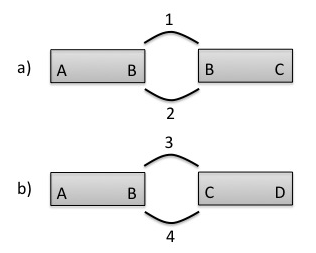
\includegraphics[scale=0.4]{./img/modelagem_arcos}
\end{figure}


Em a) os voos respeitam a restrição geográfica, dessa forma apenas os arcos de
tipo 1 e 2 precisam ser modelados uma vez que não teria sentido fazer um voo de
reposicionamento nessa situação. Em b) os aeroportos em questão são diferentes,
sendo necessário apenas a modelagem dos arcos do tipo 3 e 4, perceba que não
teria outra saída se não efetuar um voo de reposicionamento.


Seja $D = (V,A)$ um grafo representando uma instância do PCTA, onde o conjunto
de vértice $V = {v_{i}:i \in I}$ de D é indexado por $I = {1, 2, ..., n+1,
n+2}$ onde $v_{n+1}$ e $v_{n+2}$, identificam, respectivamente, os nós fonte e
destino. E os nós restantes referem-se ao conjunto de arcos originais, com $n$
elementos. Seja os custos ${c_{ij}:(i,j) \in A}$ introduzidos acima, estando
associados com cada arco da instância.
  
Seja ${x_{ij}:(i,j) \in A}$ um conjunto binário 0-1 de variáveis usada para
controlar a inclusão $(x_{ij} = 1)$ ou a exclusão $(x_{ij} = 0)$ de um arco
(possível conexão) entre vértices (voos) $v_{i}$ e $v_{j}$. O conjunto
$\overline{I}$ identifica o conjunto de nós excluindo o nó fonte $(v_{n+1})$ e
o nó de destino $(v_{n+2})$. Variáveis reais $\delta_{i}$ e $\theta_{i}$, $i
\in \overline{I}$ são usados para representar, respectivamente, o desvio do
tempo de partida sugerido e a norma desse desvio para $v_{i}$. Essas variáveis
devem no entanto obedecer $-\gamma_{i} \geq \delta_{i} \geq \gamma_{i}$ e $0
\geq \theta_{i} \geq \gamma_{i}$, onde $\gamma_{i}$ é o valor máximo de desvio
permitido (em cada direção) do tempo de partida sugerido para o voo. Finalmente
o tempo de partida sugerido que é dado por $s_{i}:i \in \overline{I}$.
  
\section{Função objetivo}

\begin{equation}
Minimizar \   \ \sum_{i \in I} \sum_{j \in I} x_{ij}c_{ij} + \sum_{i \in \overline{I}} \theta_{i}
\end{equation}

\section{Restrições}

\begin{enumerate}


\item[a)] Garantia de recobrimento dos voos \\
\begin{equation}
  \sum_{i \in I} x_{ij}= 1 \   \ \forall_{j} \in \overline{I} 
\end{equation}
\begin{equation}
\sum_{j \in I} x_{ij} = 1 \   \ \forall_{i} \in \overline{I}
\end{equation}





\item[b)] Viabilidade das conexões \\
\begin{equation}
s_{i} + t_{i}x_{ij} - INF(1 - x_{ij}) + \delta_{i} \leq s_{j} + \delta_{j} \   \ \forall_{i,j} \in \overline{I}
\end{equation}
%\begin{equation}
%\sum_{i \in I} x_{i(n+1)} = 0
%\end{equation}
%\begin{equation}
%\sum_{j \in I} x_{(n+2)j} = 0
%\end{equation}

\item[c)] Modulo do desvio do tempo de partida sugerido \\
\begin{equation}
\theta_{i} \geq \delta_{i} \   \ \forall_{i} \in \overline{I}
\end{equation}
\begin{equation}
\theta_{i} \geq -\delta_{i} \   \ \forall_{i} \in \overline{I}
\end{equation}

\item[d)] Limites das variáveis \\
\begin{equation}
-\gamma_{i} \geq \delta_{i} \geq \gamma_{i} \   \ \forall_{i} \in \overline{I}
\end{equation}
\begin{equation}
0 \geq \theta_{i} \geq \gamma_{i} \   \ \forall{i} \in \overline{I}
\end{equation}
\end{enumerate}

\clearpage

Pode-se perceber que o modelo matemático não faz menção ao tempo de solo ($g$),
isso ocorre porque esse tempo é incorporado ao voo como demonstrado na Figura
\ref{fig:conversion}, ou seja o tempo de partida sugerido $s$ passa a ter o
valor $s - g$ e a duração $t$ do voo passa a ter o valor $t + g$. Uma vantagem
de usar essa abordagem que integra o tempo de solo ao voo é que a quantidade de
restrições é reduzida.

\begin{figure}[ht]
	\centering
	\caption{Conversão de um voo para ser utilizado no
	solver. \mbox{Fonte: (Própria)}}\label{fig:conversion}
	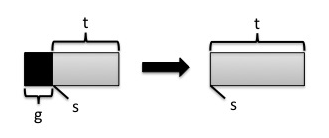
\includegraphics[scale=0.4]{./img/conversion}
	
\end{figure}

Além disso o conjunto $A$ contém apenas um tipo de arco, o arco do tipo 1 se os
voos satisfazem a restrição geográfica e o arco do tipo 3 caso não satisfaçam.
Os arcos do tipo 2 e 4 são modelados a partir  da variável $\delta$ que tem seu
custo acrescentado na função objetivo.

Essa estratégia permite a redução de 3 arcos para cada voo, o que deixa o
modelo mais leve.

O calculo dos custos são feitos através de um pré-processamento, onde os arcos
viáveis recebem os valores referentes ao seu tipo, por exemplo, no caso de um
arco originário do nó source, arco do tipo 6, um custo 1000 é atribuído. No
caso de arcos que deverão ser evitados um custo elevado é atribuído.
  	
  
\section{Fase de construção}
  
  A construção da solução é feita elemento a elemento utilizando o
  GRASP. A primeira coisa a se fazer é ordenar o conjunto de voos a partir do
  seu tempo de partida sugerido. O algoritmo só termina quando todos os voos já
  foram alocados em algum trilho.
  
  Existe duas formas de fazer a montagem da solução, uma seria a montagem
  trilho a trilho, onde um novo trilho só poderia ser criado quando o anterior
  já estivesse saturado. A outra forma é a montagem de trilhos de forma
  paralela, que, a priori, provocaria uma melhor distribuição dos voos. Na
  prática a primeira abordagem é adotada, pois, nas instâncias disponíveis ela
  apresentou, sempre, soluções de melhores qualidades. Uma maior quantidade de
  testes ainda é necessário para decidir qual a abordagem deverá ser utilizada
  ou se deverá, por exemplo, ser feita uma alteração na estratégia escolhida de
  acordo com alguma característica da instância.
  
\subsection{Formação dos trilhos de forma sequencial}

Quando se pensa na escolha do primeiro voo do trilho a decisão imediata é a
escolha do voo que contenha o menor horário de partida sugerido. Porém essa
escolha reduz a quantidade de soluções que podem ser geradas, pois a escolha
dos voos restantes do trilho é diretamente influenciada pela escolha do voo
inicial.

A abordagem utilizada para a escolha do primeiro voo inicia com a criação de
uma lista de candidatos iniciais (LCI) que é formada pelos 5 voos com os menores
horários de partida sugerido que ainda não foram alocados em nenhum outro
trilho. A escolha do voo inicial é feita de forma aleatória entre os elementos da LCI.


\subsection{Formação dos trilhos de forma paralela}
  
Essa estratégia monta uma conjunto de trilhos e constroi eles de forma
paralela. Em cada iteração o trilho corrente é escolhido a partir desse
conjunto de forma aleatória. O passo seguinte é a adição de um voo a esse
trilho ou a sua remoção do conjunto de trilhos que estão em construção, esse
segundo caso ocorre quando a lista de candidatos para esse trilho é vazia.
  
\subsection{Escolha dos voos de um trilho}

A escolha do primeiro voo de um trilho é feita como explicado nas seções
anteriores. A escolha dos demais voos é feita com base no tipo de arco e na
lista restrita de candidatos.
 
Os tipos de arcos foram definidos no Capítulo \ref{cap:descprob}, porém nessa
etapa apenas 4 tipos são considerados, o   $A_{1},A_{2},A_{3},A_{4}$ que
representam formas de ligações entre os voos. Os arcos do tipo 5 e 6 só são
utilizados apenas na modelagem matemática. Os arcos do tipo 1 permitem a
ligação de voos sem a utilização de atrasos e/ou reposicionamentos. Os arcos do
tipo 2 utilizam atrasos mas não o reposicionamento. Os arcos do tipo 3 permitem
o sequenciamento com a utilização de um voo de reposicionamento mas sem inserir
atraso em nenhum dos voos envolvidos. Os arcos do tipo 4 utilizam-se de atrasos
e de um voo de reposicionamento para fazer a ligação entre dois voos. Os arcos
do tipo 5 pargem do nó \textit{source} e servem para modelar o inicio de um
trilho. Os arcos do tipo 6 tem chegam ao nó \textit{sink} e indicam o fim de um
trilho.
 
O primeiro passo na escolha de um voo é a definição do tipo de arco que irá ser
utilizado. Essa escolha é feita tendo como base as probabilidades 0.79, 0.16,
0.04, 0.01 quer representam respectivamente os arcos do tipo 1 a 4. Esses
valores foram obtidos a partir da porcentagem dos tipos de arcos presentes em
uma solução ótima de um problema real.
 
De posse do tipo de arco, é feita então a formação da lista de candidatos. Essa
lista é ordenada de acordo com o seu horário de partida sugerido, caso o arco
seja do tipo $A_{1}$, ou pelo custo associado a sua escolha para os demais
tipos de arco. No caso da lista de candidatos não possuir nenhum voo, então
outro tipo de arco é sorteado, até que não seja possível acrescentar nenhum voo
ao trilho. Quando isso ocorre a construção desse trilho é finalizada.
 
Caso seja possível a obtenção de uma lista de candidatos então ela é reduzida
tendo como base o passo 4 a 6 do algoritmo \ref{alg:graspcons}. Como está lista
se encontra ordenada, então, o elemento de menor impacto ($v_{menor}$) na
solução é o primeiro e o de maior impacto ($v_{maior}$) é o último. Dessa forma
o elemento escolhido poderá ter o seu valor de impacto na solução de até
$valor_{menor} + \alpha*(valor_{maior} + valor_{menor})$. O valor de $\alpha$
ainda é objeto de estudo, mas bons resultados tem sido obtido para $\alpha$
igual a 0.5.
 
 \section{Fase de busca local}
 
A fase de busca local recebe uma solução e tem como objetivo melhora-la. No
método proposto essa fase foi substituída pelo ILS. Ou seja primeiro são
aplicados as estruturas de vizinhança, visando obter o valor ótimo local da
solução. Depois é feita uma perturbação que diversifica melhorando o valor da
função objetivo. Quando nenhuma das duas estratégias consegue melhorar a
solução então a busca local encerra e uma nova iteração do GRASP pode ser
iniciada.
 
 \subsection{Vizinhança}
 
Foram definidas 3 estruturas de vizinhança, o Swap-X e o Cross-Over, que tem o
objetivo de remover modificações nos horários de partida sugeridos dos voos, e
a Compactação, que promove a redução do número de trilhos. Abaixo essa
estruturas são explicadas.
 
\subsubsection{Swap-X}

Esse operador efetua a troca de X voos de um trilho por um conjunto de voos de
outro trilho. No método proposto apenas os movimentos do tipo Swap-1 e Swap-2
são utilizados, pois essa vizinhança é considerada grande. Na Figura X um caso
de melhoria no custo dos trilhos é exemplificada.
 
 \subsubsection{Cross-Over}
 
A ideia do operador $crossover$ é a de efetuar troca entre dois segmentos de
trilhos com a finalidade de gerar novos trilhos com menos modificações no
horário de partida. A Figura X ilustra uma melhoria causada por um movimento
desse tipo.
 
 \subsubsection{Compactação}
 
A compactação é a única estrutura de vizinhança utilizada que é capaz de
reduzir a quantidade de trilhos da solução final.
 
Isso ocorre porque ela consegue, insere um trilho em outro de forma direta ou
com a utilização de um voo de reposicionamento.
 
A figura X mostra a redução de um trilho com a utilização desse movimento.
 
 \subsection{Perturbação usando o método exato}
   
A perturbação normalmente é utilizada quando as estruturas de vizinhança não
conseguem melhorar a solução. Quando isso ocorre pode-se dizer que a solução
corrente é a ótima local com relação a vizinhança definida.
 
Para tentar encontrar outros mínimos locais aplica-se uma modificação na
estrutura da solução, mesmo que isso provoque uma piora na sua qualidade, e
depois procura-se melhora-la aplicando novamente uma busca local.
 
O método de perturbação utilizado aqui difere do que normalmente é aplicado
pois a solução, apesar de ter sua estrutura modificada, ainda consegue melhorar
a sua qualidade.
 
A sua utilização ocorre com a seleção de um conjunto de trilhos, que juntos
definem um subproblema, e a posterior aplicação de um método exato no conjunto
de voos que os formam. O método exato irá retornar a configuração ótima desses
voos, que serão agrupados novamente a solução antiga. A seleção dos trilhos é
feita com base no seu \textit{grau de compactação}. O grau de compactação é
definido como sendo a porcentagem de utilização efetiva de um trilho com
relação ao tempo de partida do primeiro voo e o tempo de chegada do ultimo voo
da instância. O calculo do grau de compactação não leva em consideração os voos
de reposicionamento, pois eles não são passados para o modelo.
 
Os trilhos são adicionados a solução até o limite de 80 voos, pois o solver
consegue, de forma imediata, resolver um problema desse porte.
	
Foram estudadas 3 formas de adicionar os trilhos ao solver:
	
	\begin{itemize}
\item Adição dos trilhos com maior grau de compactação.
\item Adição dos trilhos com menor grau de compactação.
\item Alternar entre a adição de um trilho com maior grau de compactação e outro com o menor grau de compactação.
\end{itemize}
 
 A utilização da segunda abordagem proporcionou melhores resultados.
 
 